\documentclass[a4paper,11pt]{article}
\usepackage[dutch]{babel}
\usepackage{listings}
\usepackage{xcolor}
\usepackage{graphicx}
\usepackage{geometry}
\usepackage{pgfplots}
\pgfplotsset{compat=1.18}
\geometry{margin=2.5cm}

% RISC-V assembly syntax highlighting
\lstdefinestyle{riscv}{
    language=[x86masm]Assembler,
    basicstyle=\ttfamily\small,
    keywordstyle=\color{blue}\bfseries,
    commentstyle=\color{green!60!black},
    stringstyle=\color{red},
    numbers=left,
    numberstyle=\tiny\color{gray},
    stepnumber=1,
    numbersep=5pt,
    backgroundcolor=\color{gray!5},
    frame=single,
    breaklines=true,
    captionpos=b
}

\title{Taak 2: RISC-V Assembly Programming}
\author{Benjamin}
\date{\today}

\begin{document}

\maketitle

\section{Oefening 1: String Omkeren}

\subsection{Volledige Code met Uitleg}

\subsubsection{1. Data Sectie}
\begin{lstlisting}[style=riscv]
.data
lab:
    .byte 'p'
    .byte 'a'
    .byte 'n'
    .byte 'n'
    .byte 'e'
    .byte 'k'
    .byte 'o'
    .byte 'e'
    .byte 'k'
    .byte 0             # null-terminator
\end{lstlisting}
\textbf{Uitleg} : pannekoek staat per byte in geheugen de 0 geeft aan waar de string eindigt.
\subsubsection{2. Programma Start en Originele Printen}
\begin{lstlisting}[style=riscv]
.text
.globl _start

_start:
    # Print de originele string
    la t0, lab          # laad adres string in t0
    jal print_string    # roep print functie aan
\end{lstlisting}

\textbf{Uitleg:} Het programma start door het adres van de string te laden en de \texttt{print\_string} functie aan te roepen.

\subsubsection{3. Hulpfunctie: print\_string}
\begin{lstlisting}[style=riscv]
print_string:
print_loop:
    lb a1, 0(t0)        # laad karakter in a1
    beq a1, x0, print_end  # als null, stop
    li a0, 11           # syscall ID = print character
    ecall
    addi t0, t0, 1      # volgende karakter 
    j print_loop

print_end:
    ret                 # return naar caller
\end{lstlisting}

\textbf{Uitleg:} Deze functie print een null-terminated string vanaf het adres in \texttt{t0}. Het loopt door elk karakter tot de null-terminator.

\subsubsection{4. Lengteberekening}
\begin{lstlisting}[style=riscv]
    # Bereken lengte van string
    la t0, lab          # begin adres van string
    li t1, 0            # teller voor lengte

lengte_berekenen:
    add t2, t0, t1      # adres van huidig karakter
    lb t3, 0(t2)        # laad karakter
    beq t3, x0, print_omgekeerd  # als null, start omgekeerd printen
    addi t1, t1, 1      # lengte++
    j lengte_berekenen
\end{lstlisting}

\textbf{Uitleg:} De lengte wordt berekend door elk karakter te tellen tot de null-terminator wordt bereikt. Register \texttt{t1} houdt de teller bij en bevat uiteindelijk de lengte

\subsubsection{5. Omgekeerd Printen}
\begin{lstlisting}[style=riscv]
print_omgekeerd:
    # Print de omgekeerde string (van einde naar begin)
    addi t1, t1, -1     # t1 = laatste index (lengte - 1)
    la t0, lab          # begin adres van string

print_omgekeerd_loop:
    blt t1, x0, end_program  # als index < 0, klaar
    
    add t2, t0, t1      # adres van karakter op positie t1
    lb a1, 0(t2)        # laad karakter in a1
    li a0, 11           # syscall ID = print character
    ecall
    
    addi t1, t1, -1     # ga naar vorig karakter
    j print_omgekeerd_loop
\end{lstlisting}

\textbf{Uitleg:} De string wordt omgekeerd geprint door te beginnen bij het laatste karakter (index = lengte-1) en terug te tellen naar index 0. Elk karakter wordt individueel geprint met syscall 11.

\subsubsection{6. Programma Afsluiten}
\begin{lstlisting}[style=riscv]
end_program:
    li a0, 10           # syscall ID = exit
    ecall
\end{lstlisting}

\textbf{Uitleg:} Het programma wordt afgesloten met syscall 10 (exit).

\subsection{Terminal Output}
\begin{figure}[h]
    \centering
    \fbox{%
        \parbox{0.8\textwidth}{%
            \centering
            % Plaats hier je screenshot
            \includegraphics[width=0.75\textwidth]{fotos/screenshot_oef1.png}
            
            % OF als je nog geen screenshot hebt, gebruik deze placeholder:
            % \vspace{3cm}
            % \textit{[Screenshot van terminal output]}
            % \vspace{3cm}
        }
    }
    \label{fig:output}
\end{figure}


\section{Oefening 2: Bubblesort en Mediaan}

\subsection{Probleemstelling}
Sorteer een array van 101 integers met bubblesort en bereken de mediaan. We vergelijken een basis implementatie met een geoptimaliseerde versie.

\subsection{Data Sectie en Initialisatie (Identiek in beide versies)}

\begin{lstlisting}[style=riscv]
.data
    lengte: .word 101
    array: .word 1036, 783, 710, ...  # 101 elementen

.text
.globl _start

_start:
    la t0, lengte       # laad adres lengte
    lw t1, 0(t0)        # t1 = 101 (aantal elementen)
    la t2, array        # t2 = begin adres array
    
    # Print originele array (code identiek in beide versies)
\end{lstlisting}

\subsection{Vergelijking 1: Buitenste Lus Setup}

\begin{table}[h]
\centering
\begin{tabular}{|p{7.5cm}|p{7.5cm}|}
\hline
\textbf{Basis Versie} & \textbf{Geoptimaliseerde Versie} \\ \hline
\begin{lstlisting}[style=riscv, numbers=none, basicstyle=\ttfamily\footnotesize]
li t3, 0            # i (buitenste lus)

outer_lus:
    bge t3, t1, klaar_met_sorteren
    la t2, array
    li t4, 0        # j (binnenste lus)
\end{lstlisting}
& 
\begin{lstlisting}[style=riscv, numbers=none, basicstyle=\ttfamily\footnotesize]
addi t3, t1, -1  # t3 = lengte - 1

buitenste_lus:
    blez t3, einde_buitenste_lus
    li t5, 0     # vlag voor wissel
    la t2, array
    mv t4, t3    # binnenste teller = t3
\end{lstlisting}
\\ \hline
\end{tabular}
\end{table}

\textbf{Wat is het verschil?}
\begin{itemize}
    \item \textbf{Basis:} Teller \texttt{t3} loopt van 0 tot 101. De binnenste lus doet altijd 100 vergelijkingen.
    \item \textbf{Geoptimaliseerd:} \texttt{t3} start bij 100 en vermindert elke keer. De binnenste lus doet eerst 100, dan 99, dan 98 vergelijkingen, etc.
    \item \textbf{Voordeel:} Na elke ronde is het grootste element op zijn plek. Waarom opnieuw controleren?
    \item \textbf{Extra:} \texttt{t5} is een vlag die bijhoudt of er gewisseld is (zie volgende vergelijking).
\end{itemize}

\subsection{Vergelijking 2: Binnenste Lus en Wissel Logica}

\begin{table}[h]
\centering
\begin{tabular}{|p{7.5cm}|p{7.5cm}|}
\hline
\textbf{Basis Versie} & \textbf{Geoptimaliseerde Versie} \\ \hline
\begin{lstlisting}[style=riscv, numbers=none, basicstyle=\ttfamily\footnotesize]
inner_lus:
    addi t5, t1, -1         # t5 = laatste index
    bge t4, t5, klaar_inner_lus  # klaar?
    
    lw t6, 0(t2)            # t6 = array[j]
    lw a1, 4(t2)            # a1 = array[j+1]
    blt a1, t6, doe_wissel  # a1 < t6? wissel
    j niet_wisselen         # anders skip
    
doe_wissel:
    sw a1, 0(t2)            # zet a1 op positie j
    sw t6, 4(t2)            # zet t6 op positie j+1
    
niet_wisselen:
    addi t2, t2, 4          # volgende positie
    addi t4, t4, 1          # j++
    j inner_lus             # herhaal
\end{lstlisting}
& 
\begin{lstlisting}[style=riscv, numbers=none, basicstyle=\ttfamily\footnotesize]
binnenste_lus:
    lw t6, 0(t2)     # array[j]
    lw a1, 4(t2)     # array[j+1]
    ble t6, a1, geen_wissel
    
    # Wissel de twee elementen om
    sw a1, 0(t2)
    sw t6, 4(t2)
    li t5, 1         # vlag = 1 (er is gewisseld)
    
geen_wissel:
    addi t2, t2, 4   # volgend element
    addi t4, t4, -1  # binnenste teller--
    bnez t4, binnenste_lus
\end{lstlisting}
\\ \hline
\end{tabular}
\end{table}

\textbf{Wat is het verschil?}
\begin{itemize}
    \item \textbf{Basis:} Wisselt elementen als nodig, maar houdt niet bij óf er gewisseld werd.
    \item \textbf{Geoptimaliseerd:} Zet \texttt{t5 = 1} wanneer er gewisseld wordt. Als \texttt{t5} na een volledige ronde nog steeds 0 is, betekent dit: geen enkele wissel = array is gesorteerd!
    \item \textbf{Voordeel:} We kunnen vroeg stoppen (zie volgende vergelijking).
\end{itemize}

\subsection{Vergelijking 3: Early Termination (Vroegtijdig Stoppen)}

\begin{table}[h]
\centering
\begin{tabular}{|p{7.5cm}|p{7.5cm}|}
\hline
\textbf{Basis Versie} & \textbf{Geoptimaliseerde Versie} \\ \hline
\begin{lstlisting}[style=riscv, numbers=none, basicstyle=\ttfamily\footnotesize]
klaar_inner_lus:
    addi t3, t3, 1          # i++
    j outer_lus             # herhaal outer lus

# Geen check of array gesorteerd is
# Blijft altijd doorlopen
# tot alle 101 rondes gedaan zijn
\end{lstlisting}
& 
\begin{lstlisting}[style=riscv, numbers=none, basicstyle=\ttfamily\footnotesize]
    beqz t5, einde_buitenste_lus
    # Als geen wissels: array is 
    # gesorteerd -> STOP METEEN!
    
    addi t3, t3, -1
    j buitenste_lus
\end{lstlisting}
\\ \hline
\end{tabular}
\end{table}

\textbf{Wat is het verschil?}
\begin{itemize}
    \item \textbf{Basis:} Doet altijd alle 101 rondes, ook al is de array na 5 rondes al gesorteerd.
    \item \textbf{Geoptimaliseerd:} Controleert na elke ronde: "Hebben we gewisseld?" Zo niet, we zijn klaar!
    \item \textbf{Voorbeeld:} Bij een bijna gesorteerde array kan dit 95+ rondes besparen!
    \item \textbf{Resultaat:} Tot 99\% minder werk bij al gesorteerde data.
\end{itemize}

\subsection{Vergelijking 4: Mediaanberekening}

\begin{table}[h]
\centering
\begin{tabular}{|p{7.5cm}|p{7.5cm}|}
\hline
\textbf{Basis Versie} & \textbf{Geoptimaliseerde Versie} \\ \hline
\begin{lstlisting}[style=riscv, numbers=none, basicstyle=\ttfamily\footnotesize]
# Check even/oneven
andi t3, t1, 1  # lengte & 1
# Bitwise AND: laatste bit
# 1 = oneven, 0 = even
bnez t3, oneven_mediaan

# Bereken middelste positie
srli t4, t1, 1          # / 2
slli t4, t4, 2          # * 4
add t2, t2, t4
lw a0, 0(t2)
\end{lstlisting}
& 
\begin{lstlisting}[style=riscv, numbers=none, basicstyle=\ttfamily\footnotesize]
# Check even/oneven
andi t3, t1, 1  # lengte & 1
# Bitwise AND: laatste bit
# 1 = oneven, 0 = even
bnez t3, oneven_mediaan

# Bereken middelste positie
srli t4, t1, 1          # / 2
slli t4, t4, 2          # * 4
add t2, t2, t4
lw a0, 0(t2)
\end{lstlisting}
\\ \hline
\end{tabular}
\end{table}

\textbf{Wat is het verschil?}
\begin{itemize}
    \item \textbf{Basis en Geoptimaliseerd:} Beide versies gebruiken dezelfde benadering met \texttt{andi} (even/oneven check) en \texttt{srli/slli} (shift operaties).
    \item \textbf{Shift uitleg:} \texttt{srli} (shift right) = delen door 2, \texttt{slli} (shift left) = vermenigvuldigen met 2.
    \item \textbf{Even vs Oneven:} Bij oneven arrays (zoals 101 elementen) wordt het middelste element genomen. Bij even arrays wordt het gemiddelde van de twee middelste elementen berekend.
\end{itemize}

\subsection{Performance Vergelijking}

De geoptimaliseerde versie presteert beter dan de basis implementatie. De grootste winst wordt behaald wanneer de data al (bijna) gesorteerd is, omdat het algoritme dan vroegtijdig kan stoppen.

\begin{figure}[h]
    \centering
    \begin{minipage}{0.45\textwidth}
        \centering
        \fbox{%
            \parbox{0.95\textwidth}{%
                \centering
                \includegraphics[width=0.9\textwidth]{fotos/bubblesort_basic_cycles.png}
                
                % Placeholder:
                % \vspace{2cm}
                % \textit{[Screenshot cycles basic]}
                % \vspace{2cm}
            }
        }
        \caption{Cycle count: basis versie}
    \end{minipage}
    \hfill
    \begin{minipage}{0.45\textwidth}
        \centering
        \fbox{%
            \parbox{0.95\textwidth}{%
                \centering
                \includegraphics[width=0.9\textwidth]{fotos/bubblesort_optimized_cycles.png}
                
                % Placeholder:
                % \vspace{2cm}
                % \textit{[Screenshot cycles optimized]}
                % \vspace{2cm}
            }
        }
        \caption{Cycle count: geoptimaliseerd}
    \end{minipage}
\end{figure}

\newpage
\section{Oefening 3: Fibonacci Berekening}

\subsection{Probleemstelling}
Bereken het n-de Fibonacci getal iteratief in RISC-V assembly. De Fibonacci reeks: 0, 1, 1, 2, 3, 5, 8, 13, 21, ...

\subsection{Hoe Werkt Het?}

\textbf{De Truc:} In plaats van elke keer opnieuw te berekenen, onthouden we gewoon de laatste twee getallen en schuiven we door.

\subsubsection{Basis Gevallen}
\begin{lstlisting}[style=riscv]
fibonacci:
    li t0, 1
    ble a0, t0, fib_base_case   # Als n <= 1, return n
\end{lstlisting}

\textbf{Simpel:} F(0) = 0 en F(1) = 1. Klaar.

\subsubsection{Iteratieve Berekening}
\begin{lstlisting}[style=riscv]
    mv t0, a0           # t0 = n (hoe ver we moeten)
    li t1, 0            # t1 = F(n-2), start: F(0) = 0
    li t2, 1            # t2 = F(n-1), start: F(1) = 1
    li t3, 2            # t3 = teller, start bij 2
\end{lstlisting}

\textbf{Setup:} We beginnen met F(0)=0 en F(1)=1. Teller start bij 2 want we kennen al F(0) en F(1).

\subsubsection{De Lus}
\begin{lstlisting}[style=riscv]
fib_loop:
    bgt t3, t0, fib_done        # Klaar als i > n
    
    add t4, t1, t2              # F(i) = F(i-2) + F(i-1)
    
    mv t1, t2                   # Schuif: F(n-2) = oude F(n-1)
    mv t2, t4                   # Schuif: F(n-1) = nieuwe F(i)
    
    addi t3, t3, 1              # i++
    j fib_loop
\end{lstlisting}

\textbf{Het Idee:}
\begin{enumerate}
    \item Bereken nieuw getal: \texttt{t4 = t1 + t2}
    \item Schuif waardes door: oude F(n-1) wordt nieuwe F(n-2)
    \item Nieuw getal wordt F(n-1)
    \item Herhaal
\end{enumerate}

\textbf{Voorbeeld voor F(5):}
\begin{itemize}
    \item Start: t1=0, t2=1
    \item i=2: t4=0+1=1 → t1=1, t2=1
    \item i=3: t4=1+1=2 → t1=1, t2=2
    \item i=4: t4=1+2=3 → t1=2, t2=3
    \item i=5: t4=2+3=5 → t1=3, t2=5 ✓
\end{itemize}

\subsection{Performance Analyse}

De iteratieve methode is efficiënt: elke iteratie kost ongeveer 6 cycles (load, add, move, branch). De relatie tussen n en cycles is lineair.

\begin{figure}[h]
    \centering
    \fbox{%
        \parbox{0.8\textwidth}{%
            \centering
            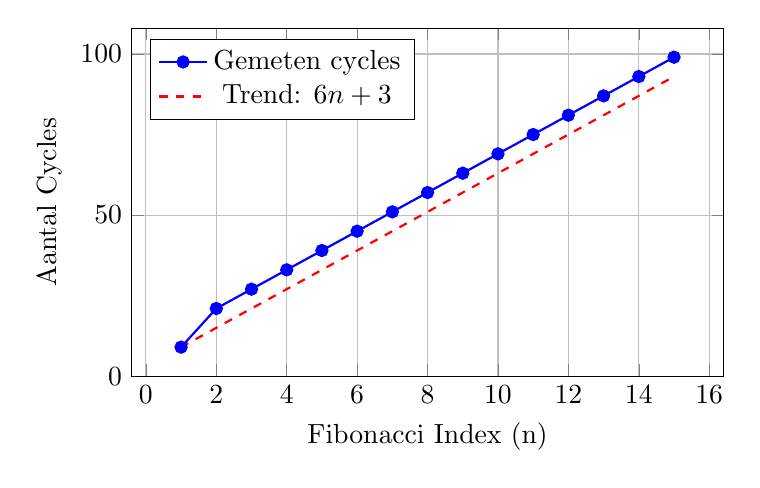
\begin{tikzpicture}
                \begin{axis}[
                    width=0.75\textwidth,
                    height=6cm,
                    xlabel={Fibonacci Index (n)},
                    ylabel={Aantal Cycles},
                    grid=major,
                    legend pos=north west,
                    ymajorgrids=true,
                    xmajorgrids=true,
                ]
                \addplot[
                    color=blue,
                    mark=*,
                    thick,
                ] coordinates {
                    (1,9) (2,21) (3,27) (4,33) (5,39) (6,45) (7,51) 
                    (8,57) (9,63) (10,69) (11,75) (12,81) (13,87) (14,93) (15,99)
                };
                \addlegendentry{Gemeten cycles}
                
                % Lineaire trend lijn
                \addplot[
                    color=red,
                    dashed,
                    thick,
                    domain=1:15,
                ] {6*x + 3};
                \addlegendentry{Trend: $6n + 3$}
                \end{axis}
            \end{tikzpicture}
        }
    }
    \caption{Cycle count versus Fibonacci index}
    \label{fig:fib_cycles}
\end{figure}

\textbf{Observaties:}
\begin{itemize}
    \item \textbf{Lineaire groei:} Elke stap kost ongeveer 6 extra cycles
    \item \textbf{Formule:} Cycles $\approx 6n + 3$ (overhead van setup + loop)
    \item \textbf{F(1) speciale case:} 9 cycles door basis case check
    \item \textbf{Efficiëntie:} O(n) tijd én O(1) geheugen - kan niet beter!
\end{itemize}

\newpage
\appendix
\section{Bijlage: Volledige Code}

Deze bijlage bevat alle volledige code die direct kan worden gekopieerd en uitgevoerd.

\subsection{Oefening 1: String Omkeren (oef1.s)}

\begin{lstlisting}[style=riscv, numbers=none]
.data
lab:
    .byte 'p'
    .byte 'a'
    .byte 'n'
    .byte 'n'
    .byte 'e'
    .byte 'k'
    .byte 'o'
    .byte 'e'
    .byte 'k'
    .byte 0

.text
.globl _start

_start:
    # Print de originele string
    la t0, lab
    jal print_string
    
    # Bereken lengte van string
    la t0, lab          # begin adres van string
    li t1, 0            # teller voor lengte

lengte_berekenen:
    add t2, t0, t1      # adres van huidig karakter
    lb t3, 0(t2)        # laad karakter
    beq t3, x0, print_omgekeerd  # als null, start omgekeerd printen
    addi t1, t1, 1      # lengte++
    j lengte_berekenen

print_omgekeerd:
    # Print de omgekeerde string (van einde naar begin)
    addi t1, t1, -1     # t1 = laatste index (lengte - 1)
    la t0, lab          # begin adres van string

print_omgekeerd_loop:
    blt t1, x0, end_program  # als index < 0, klaar
    
    add t2, t0, t1      # adres van karakter op positie t1
    lb a1, 0(t2)        # laad karakter in a1
    li a0, 11           # ecall ID = print character
    ecall
    
    addi t1, t1, -1     # ga naar vorig karakter
    j print_omgekeerd_loop

end_program:
    li a0, 10           # ecall = einde programma
    ecall


print_string:
print_loop:
    lb a1, 0(t0)        # laad karakter in a1
    beq a1, x0, print_end  # als null, stop
    li a0, 11           # ecall  = print character
    ecall
    addi t0, t0, 1      # volgende karakter (bytes!)
    j print_loop

print_end:
    ret
\end{lstlisting}

\subsection{Oefening 2: Bubblesort - Niet-geoptimaliseerde Versie (bubbelsort.s)}

\begin{lstlisting}[style=riscv, numbers=none]
.data
    lengte: .word 101
    array: .word 1036, 783, 710, 939, 21, 332, 675, 1398, 1337, 28, 633, 1317, 863, 873, 1094, 886, 1171, 393, 142, 111, 638, 919, 211, 1355, 998, 1131, 821, 930, 195, 276, 704, 330, 337, 160, 133, 1199, 1250, 471, 500, 107, 1466, 774, 644, 1198, 1, 668, 45, 370, 531, 440, 928, 989, 1191, 1310, 13, 1323, 254, 1168, 853, 77, 855, 831, 969, 1435, 716, 861, 239, 1239, 644, 304, 909, 1271, 523, 1360, 183, 917, 1094, 479, 1084, 765, 74, 1438, 1021, 1100, 1494, 600, 1401, 560, 217, 1422, 1383, 505, 1371, 549, 766, 1396, 471, 14, 132, 1082, 400

.text
.globl _start

_start:
    la t0, lengte           
    lw t1, 0(t0)            # t1 = aantal elementen
    la t2, array            # t2 = basis adres
    
    # Print originele array
    li t3, 0                # teller
print_origineel:
    bge t3, t1, klaar_print_origineel  # klaar?
    lw a0, 0(t2)            # laad element
    li a7, 1                # print integer ecall
    ecall
    addi t2, t2, 4          # volgende element
    addi t3, t3, 1          # teller++
    j print_origineel       # herhaal
    
klaar_print_origineel:
    la t2, array            # reset naar begin
    
    li t3, 0                # i (buitenste lus)
    
outer_lus:
    bge t3, t1, klaar_met_sorteren  # i >= lengte? klaar
    
    la t2, array            # reset naar begin
    li t4, 0                # j (binnenste lus)
    
inner_lus:
    addi t5, t1, -1         # t5 = laatste index
    bge t4, t5, klaar_inner_lus  # klaar?
    
    # Vergelijk array[j] en array[j+1]
    lw t6, 0(t2)            # t6 = array[j]
    lw a1, 4(t2)            # a1 = array[j+1]
    
    # Als array[j] > array[j+1], wissel
    blt a1, t6, doe_wissel  # a1 < t6? wissel
    j niet_wisselen         # anders skip
    
doe_wissel:
    sw a1, 0(t2)            # zet a1 op positie j
    sw t6, 4(t2)            # zet t6 op positie j+1
    
niet_wisselen:
    addi t2, t2, 4          # volgende positie
    addi t4, t4, 1          # j++
    j inner_lus             # herhaal
    
klaar_inner_lus:
    addi t3, t3, 1          # i++
    j outer_lus             # herhaal outer lus
    
klaar_met_sorteren:
    # Print gesorteerde array
    la t2, array            # reset naar begin
    li t3, 0                # reset teller
    
print_gesorteerd:
    bge t3, t1, klaar_print_gesorteerd  # klaar?
    lw a0, 0(t2)            # laad element
    li a7, 1                # print ecall 
    ecall
    addi t2, t2, 4          # volgende element
    addi t3, t3, 1          # teller++
    j print_gesorteerd      # herhaal
    
klaar_print_gesorteerd:
    # Bereken mediaan
    la t2, array            # reset naar begin
    la t0, lengte
    lw t1, 0(t0)            # Laad lengte opnieuw
    
    # Controleer of lengte even of oneven is
    andi t3, t1, 1          # t3 = lengte & 1 (geeft 1 als oneven, 0 als even)
    
    bnez t3, oneven_mediaan # Als oneven, spring naar oneven_mediaan
    
even_mediaan:
    srli t4, t1, 1          # t4 = lengte / 2
    addi t4, t4, -1         # t4 = (lengte / 2) - 1 (index eerste middelste)
    slli t4, t4, 2          # t4 = index * 4 (byte offset)
    add t2, t2, t4          # t2 = adres van eerste middelste element
    
    lw t5, 0(t2)            # t5 = array[lengte/2 - 1]
    lw t6, 4(t2)            # t6 = array[lengte/2]
    add t5, t5, t6          # t5 = som van twee middelste elementen
    srli a0, t5, 1          # a0 = gemiddelde (som / 2)
    j print_mediaan
    
oneven_mediaan:
    srli t4, t1, 1          # t4 = lengte / 2 (middelste index)
    slli t4, t4, 2          # t4 = index * 4 (byte offset)
    add t2, t2, t4          # t2 = adres van middelste element
    lw a0, 0(t2)            # a0 = mediaan waarde

print_mediaan:
    li a7, 1                # print  ecall
    ecall
    
einde:
    li a7, 10               # exit ecall
    ecall
\end{lstlisting}

\subsection{Oefening 2: Bubblesort - Geoptimaliseerde Versie (Calculatemedian.s)}

\begin{lstlisting}[style=riscv, numbers=none]
.data
    lengte: .word 101
    array: .word 1036, 783, 710, 939, 21, 332, 675, 1398, 1337, 28, 633, 1317, 863, 873, 1094, 886, 1171, 393, 142, 111, 638, 919, 211, 1355, 998, 1131, 821, 930, 195, 276, 704, 330, 337, 160, 133, 1199, 1250, 471, 500, 107, 1466, 774, 644, 1198, 1, 668, 45, 370, 531, 440, 928, 989, 1191, 1310, 13, 1323, 254, 1168, 853, 77, 855, 831, 969, 1435, 716, 861, 239, 1239, 644, 304, 909, 1271, 523, 1360, 183, 917, 1094, 479, 1084, 765, 74, 1438, 1021, 1100, 1494, 600, 1401, 560, 217, 1422, 1383, 505, 1371, 549, 766, 1396, 471, 14, 132, 1082, 400

.text
.globl _start

_start:
    la t0, lengte           # t0 = adres lengte variabele
    lw t1, 0(t0)            # t1 = lengte array (aantal elementen)
    la t2, array            # t2 = basis adres array
    
    # Print originele array 
    li t3, 0                # t3 = teller
print_origineel_lus:
    bge t3, t1, print_origineel_klaar
    lw a0, 0(t2)            
    li a7, 1                # Print integer
    ecall
    addi t2, t2, 4          # Volgende element
    addi t3, t3, 1          # Verhoog teller
    j print_origineel_lus
    
print_origineel_klaar:
    la t2, array            # Resetten 

    addi t3, t1, -1         # t3 = lengte - 1 (teller voor buitenste lus)
    
buitenste_lus:
    blez t3, einde_buitenste_lus    # t3 <= 0,klaar met sorteren
    li t5, 0                         # t5 = vlag (0 = geen wissel)
    la t2, array                     # Zet t2 terug naar begin van array
    mv t4, t3                        # t4 = teller voor binnenste lus
    
binnenste_lus:
    lw t6, 0(t2)            # t6 = array[j] (huidig element)
    lw a1, 4(t2)            # a1 = array[j+1] (volgend element)
    ble t6, a1, geen_wissel # Als array[j] <= array[j+1], geen wissel nodig
    
    # Wissel de twee elementen om
    sw a1, 0(t2)            # Zet array[j+1] op positie j
    sw t6, 4(t2)            # Zet array[j] op positie j+1
    li t5, 1                # Zet register op 1
    
geen_wissel:
    addi t2, t2, 4          # volgend element (+ 4 bytes)
    addi t4, t4, -1         # Verminder binnenste teller
    bnez t4, binnenste_lus  # Herhaal binnenste lus als t4 != 0
    
    beqz t5, einde_buitenste_lus    
    addi t3, t3, -1                  # Verminder buitenste teller
    j buitenste_lus                  # Herhaal buitenste lus
    
einde_buitenste_lus:

    # Print gesorteerde array
    la t2, array            # Reset naar begin van array
    la t0, lengte
    lw t1, 0(t0)            # t1 = lengte
    li t3, 0                # t3 = teller
    
print_lus:
    bge t3, t1, print_klaar
    lw a0, 0(t2)            # Laad array element
    li a7, 1                # Print integer
    ecall
    addi t2, t2, 4          # Volgende element
    addi t3, t3, 1          # Verhoog teller
    j print_lus
    
print_klaar:
    la t2, array            # Reset naar begin van array
    la t0, lengte
    lw t1, 0(t0)            # Laad lengte opnieuw
    
    # Controleer of lengte even of oneven is
    andi t3, t1, 1          # t3 = lengte & 1 (geeft 1 als oneven, 0 als even)
    
    bnez t3, oneven_mediaan # Als oneven, spring naar oneven_mediaan
    
even_mediaan:
    srli t4, t1, 1          # t4 = lengte / 2
    addi t4, t4, -1         # t4 = (lengte / 2) - 1 (index eerste middelste)
    slli t4, t4, 2          # t4 = index * 4 (byte offset)
    add t2, t2, t4          # t2 = adres van eerste middelste element
    
    lw t5, 0(t2)            # t5 = array[lengte/2 - 1]
    lw t6, 4(t2)            # t6 = array[lengte/2]
    add t5, t5, t6          # t5 = som van twee middelste elementen
    srli a1, t5, 1          # a1 = gemiddelde (som / 2)
    j print_mediaan
    
oneven_mediaan:
    srli t4, t1, 1          # t4 = lengte / 2 (middelste index)
    slli t4, t4, 2          # t4 = index * 4 (byte offset)
    add t2, t2, t4          # t2 = adres van middelste element
    lw a0, 0(t2)            # a0 = mediaan 

print_mediaan:
    lw a0, 0(t2)            # Laad  waarde
    li a7, 1                # Print 
    ecall
    
    # Programma afsluiten
    li a7, 10               # Exit ecall
    ecall
\end{lstlisting}

\subsection{Oefening 3: Fibonacci Berekening (fibonacci.s)}

\begin{lstlisting}[style=riscv, numbers=none]
.text
.globl _start

_start:
    li a0, 10           # n = 10 (pas aan naar wens)
    
    # Roep fibonacci functie aan
    jal ra, fibonacci
    
    li a7, 1            # ecall 1 = print integer
    ecall
    
    # Exit programma
    li a7, 10           # ecall voor exit
    ecall

fibonacci:
    # Controleer basis gevallen
    li t0, 1
    ble a0, t0, fib_base_case   # Als n <= 1, return n
    
    mv t0, a0           # t0 = n (counter)
    li t1, 0            # t1 = F(n-2), start met F(0) = 0
    li t2, 1            # t2 = F(n-1), start met F(1) = 1
    li t3, 2            # t3 = i, start bij 2
    
fib_loop:
    bgt t3, t0, fib_done    # Als i > n, klaar
    
    add t4, t1, t2      # t4 = F(i-2) + F(i-1)
    
    mv t1, t2           # F(n-2) = oude F(n-1)
    mv t2, t4           # F(n-1) = nieuwe F(n)
    
    addi t3, t3, 1      # i++
    j fib_loop
    
fib_done:
    mv a0, t2           # Resultaat in a0
    ret
    
fib_base_case:
    # Als n <= 1, return n (a0 bevat al de juiste waarde)
    ret
\end{lstlisting}

\end{document}
